\section{Methods}

Our evolutionary case studies employ an extension to the DISHTINY framework for studying fraternal transitions in individuality.
Initial work with this system characterized selective pressures for cooperation with kin \citep{moreno2019toward}.
%Upcoming work extends
We have since extended the system to use the SignalGP event-driven genetic programming technique \citep{lalejini2018evolving} to control cell behaviors.
Diverse multicellular life histories evolved in SignalGP-enabled DISHTINY evolutionary trials, involving reproductive division of labor, resource sharing (including, in some treatments, endowment of offspring groups), asymmetrical within-group and inter-group phenomena mediated by cell-cell messaging, morphological patterning, gene-regulation mediated life cycles, and adaptive apoptosis \citep{dishtinygp}.

DISHTINY simulates individual cells, each of which occupies a tile on a toroidal grid.
Cells can reproduce, placing daughter cells into adjoining tiles.
We allow cells the opportunity to engage with kin in a cooperative resource-collection task (Supplementary Section \ref{sec:resourcecollection}), which can increase their individual cellular reproduction rates.
Kin groups are explicitly registered: on birth, a cell is either added to its parents group or expelled to establish a new group (Supplementary Section \ref{sec:hierarchicalnesting}).

Cells can differentiate between neighbors that are members of their kin group and neighbors that are not and alter their behavior accordingly.
Each cell %consists of
contains four SignalGP instances (all executing the same genetic program), one of which controls cell behavior with respect to each neighbor.
These instances may communicate with one another by means of intracellular messaging.
In this work, we add a fifth SignalGP instance to the DISHTINY cell.
This instance can execute special instructions to establish long-distance interconnects with other cells and engage in resource-sharing and/or message passing with those cells.
Figure \ref{fig:spiker_pointer_hardware} summarizes how SignalGP hardware is arranged within DISHTINY cells.

Long-distance interconnects are established through a developmental process, summarized in Figure \ref{fig:spiker_diagram}.
The process begins with the placement of two independent search prongs at the originating cell \ref{fig:spiker_diagram}a.
Each prong performs a random walk over the originating cell's kin group, accumulating positive or negative feedback based on tags expressed by underfoot cells \ref{fig:spiker_diagram}b.
If a prongs accumulates positive feedback too slowly, it is reset to the location of the better-scoring prong \ref{fig:spiker_diagram}c.
Once a positive feedback threshold has been reached, the best-scoring prong develops into a full-fledged connection \ref{fig:spiker_diagram}d.
At this point, the originating cell can begin exchanging messages and/or resource over the connection \ref{fig:spiker_diagram}e.
Established interconnects may be subsequently removed by either participating cell \ref{fig:spiker_diagram}f.

Full details on hardware-level instructions and event-driven environmental cues available to cells are provided in Supplementary Sections \ref{sec:neighborinstlib}, \ref{sec:neighboreventlib}, \ref{sec:interconnectinstlib}, and \ref{sec:interconnecteventlib} \cite{Moreno_Ofria_2020}.

\begin{figure}[t]
\begin{center}
%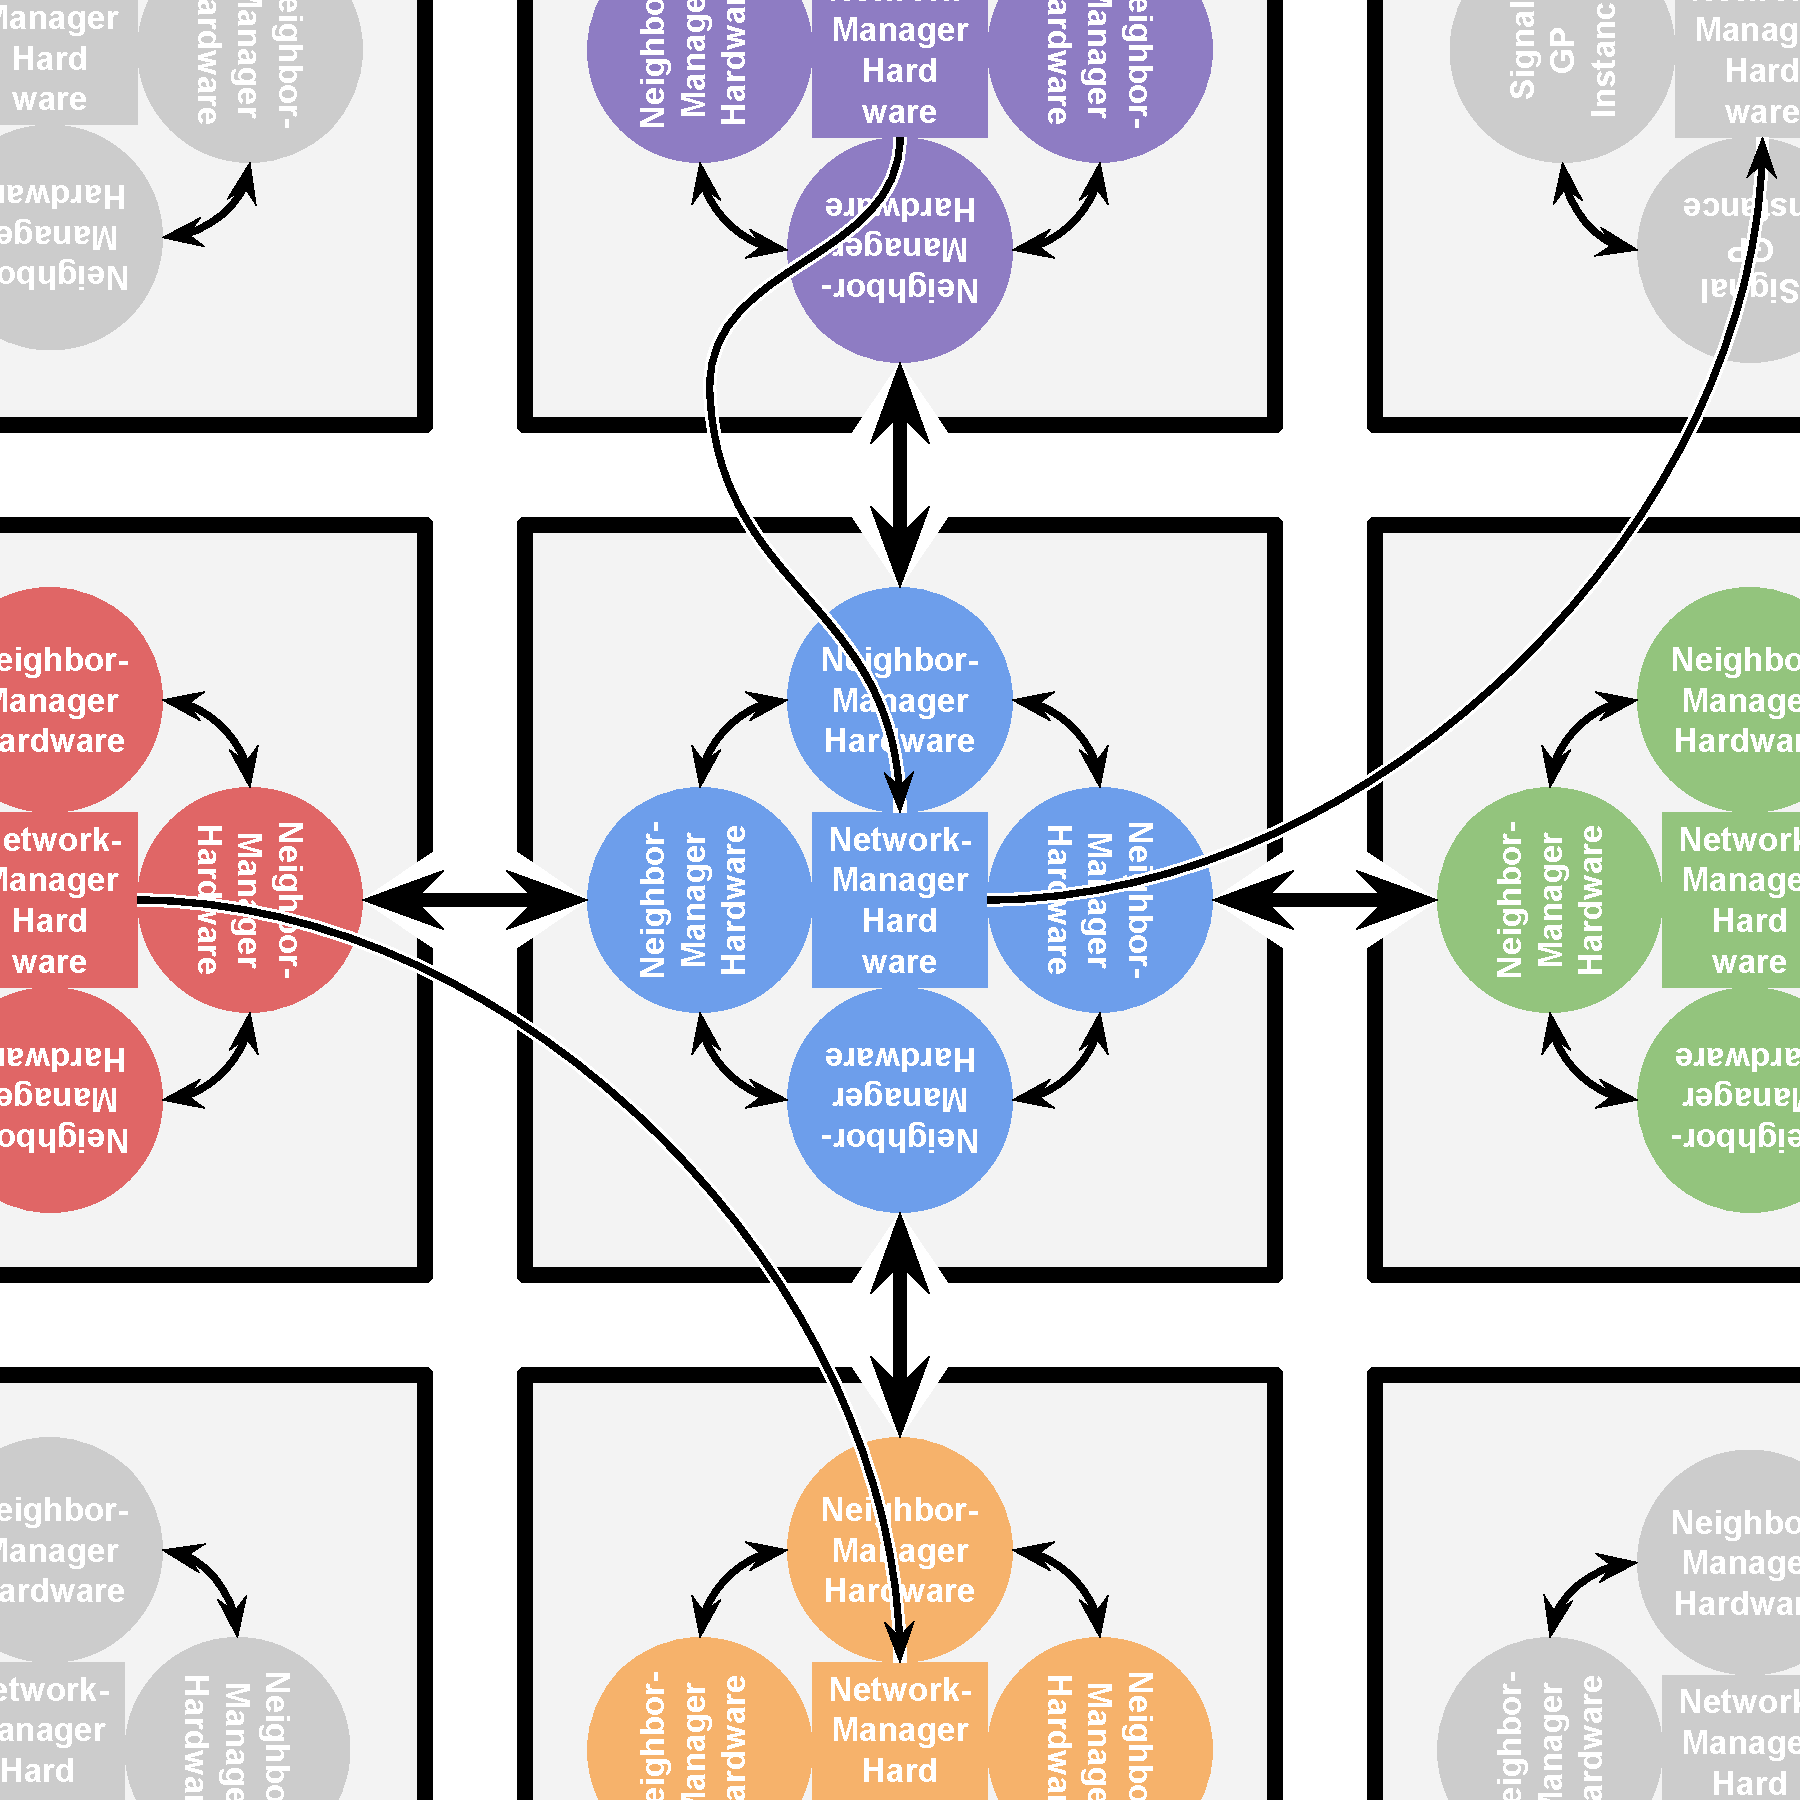
\includegraphics[width=0.7\linewidth]{img/spiker-pointer-hardware.pdf}
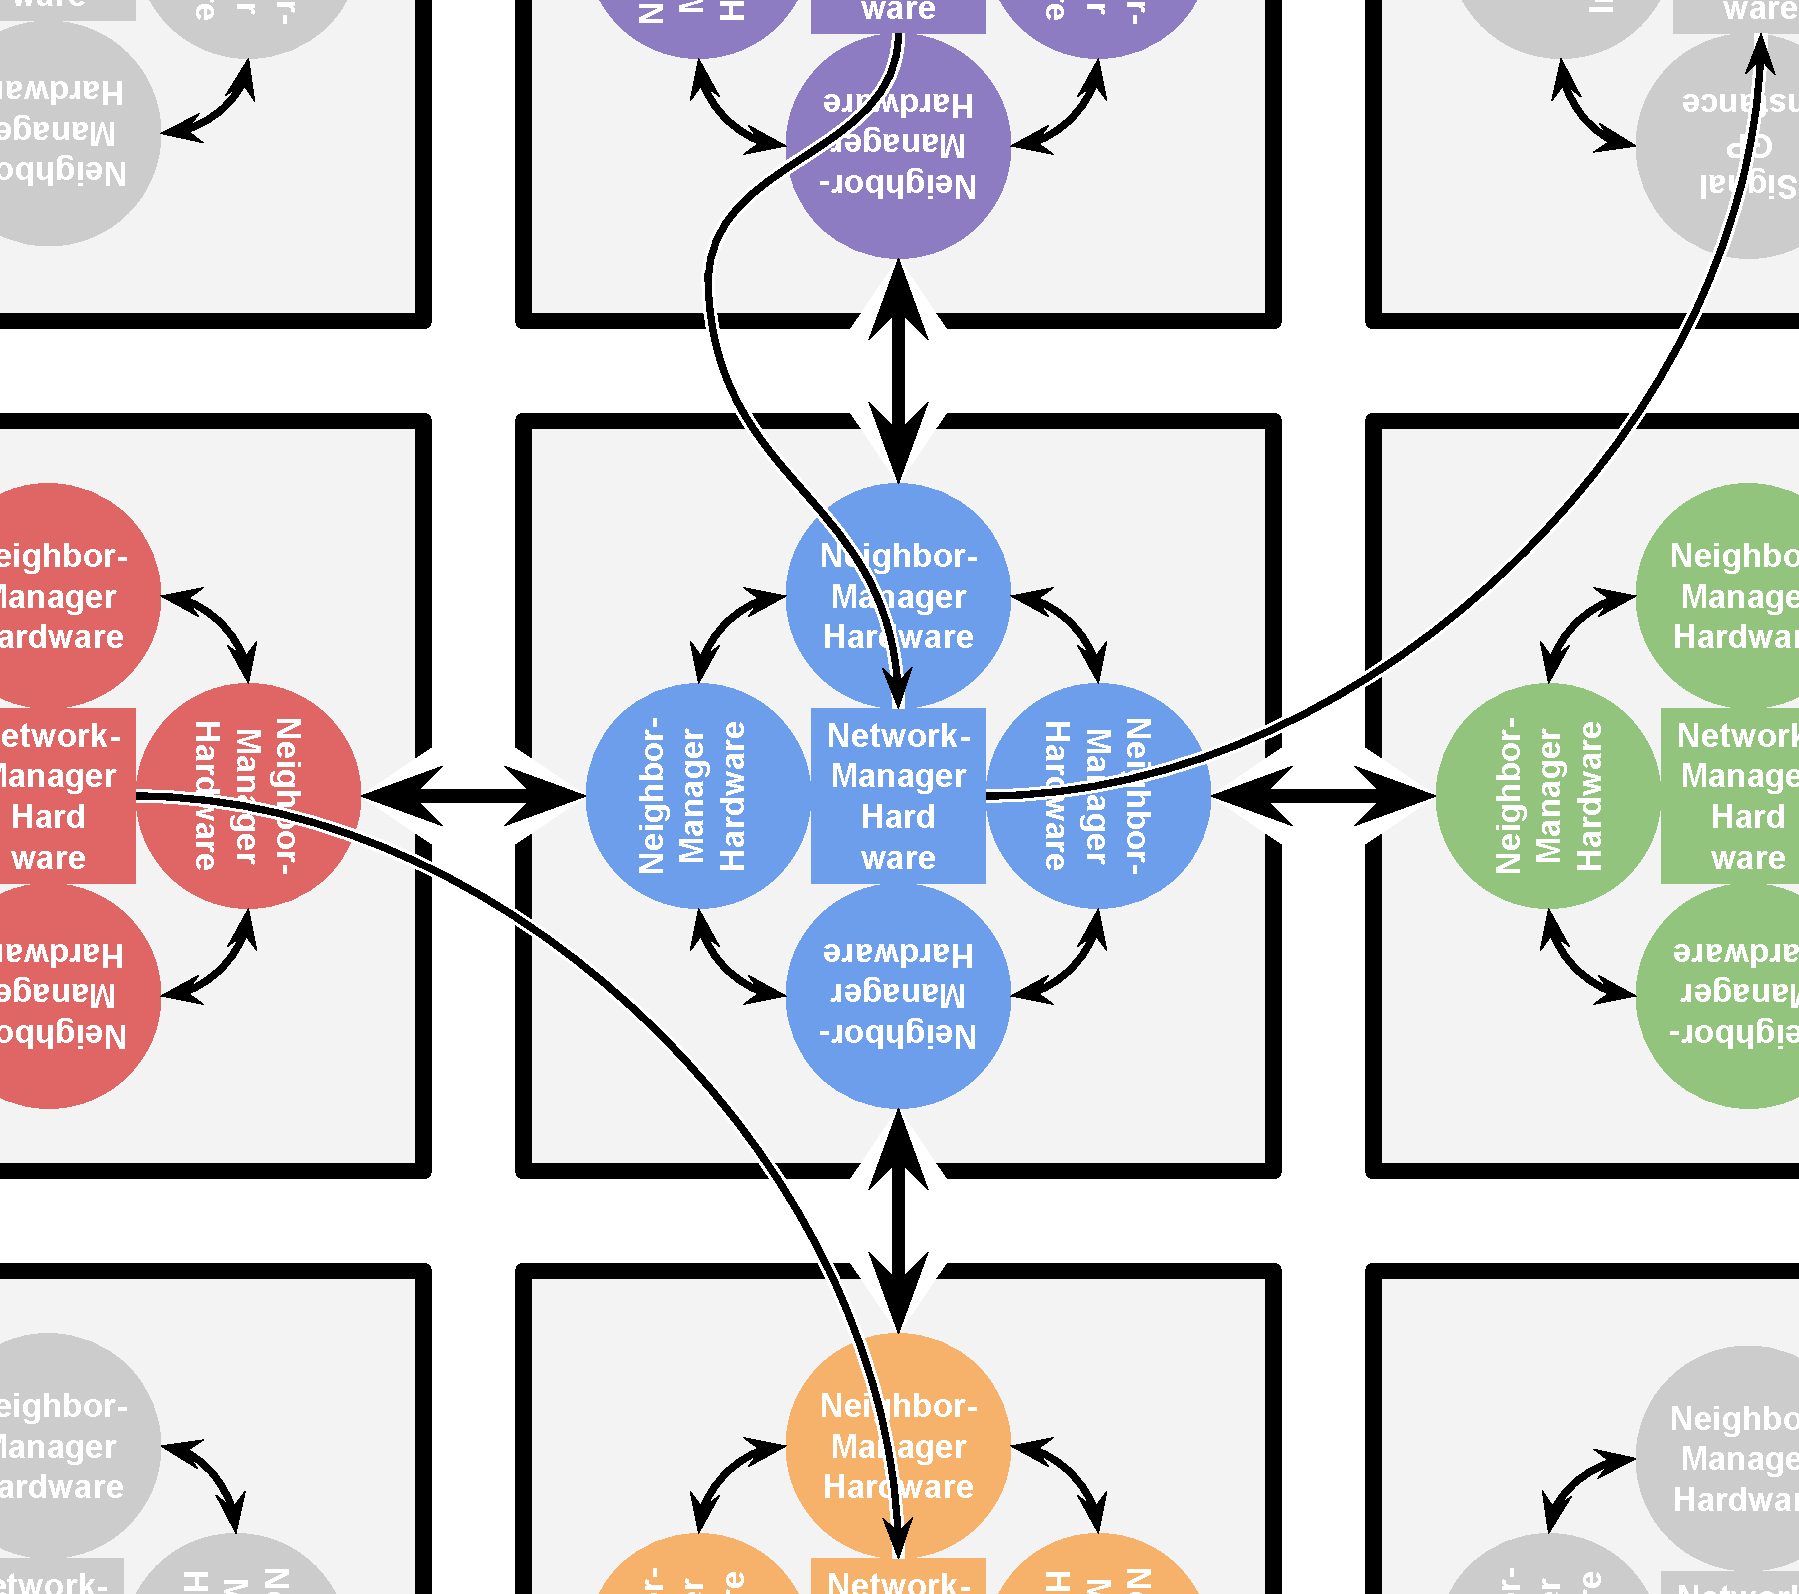
\includegraphics[width=0.8\linewidth]{img/spiker-pointer-hardware2.pdf}
\caption{
Arrangement of SignalGP hardware within DISHTINY cells (gray squares).
Neighbor-managing hardware (circles) receive stimuli and control cell behavior with respect to a particular cell neighbor.
Network-managing hardware (interior squares) receive stimuli and controll cell behavior with respect to more distant neighbors a cell has established interconnects with.
}
\label{fig:spiker_pointer_hardware}
\end{center}
\end{figure}


\begin{figure*}[!htbp]
\begin{center}
\begin{subfigure}[b]{0.33\linewidth}
  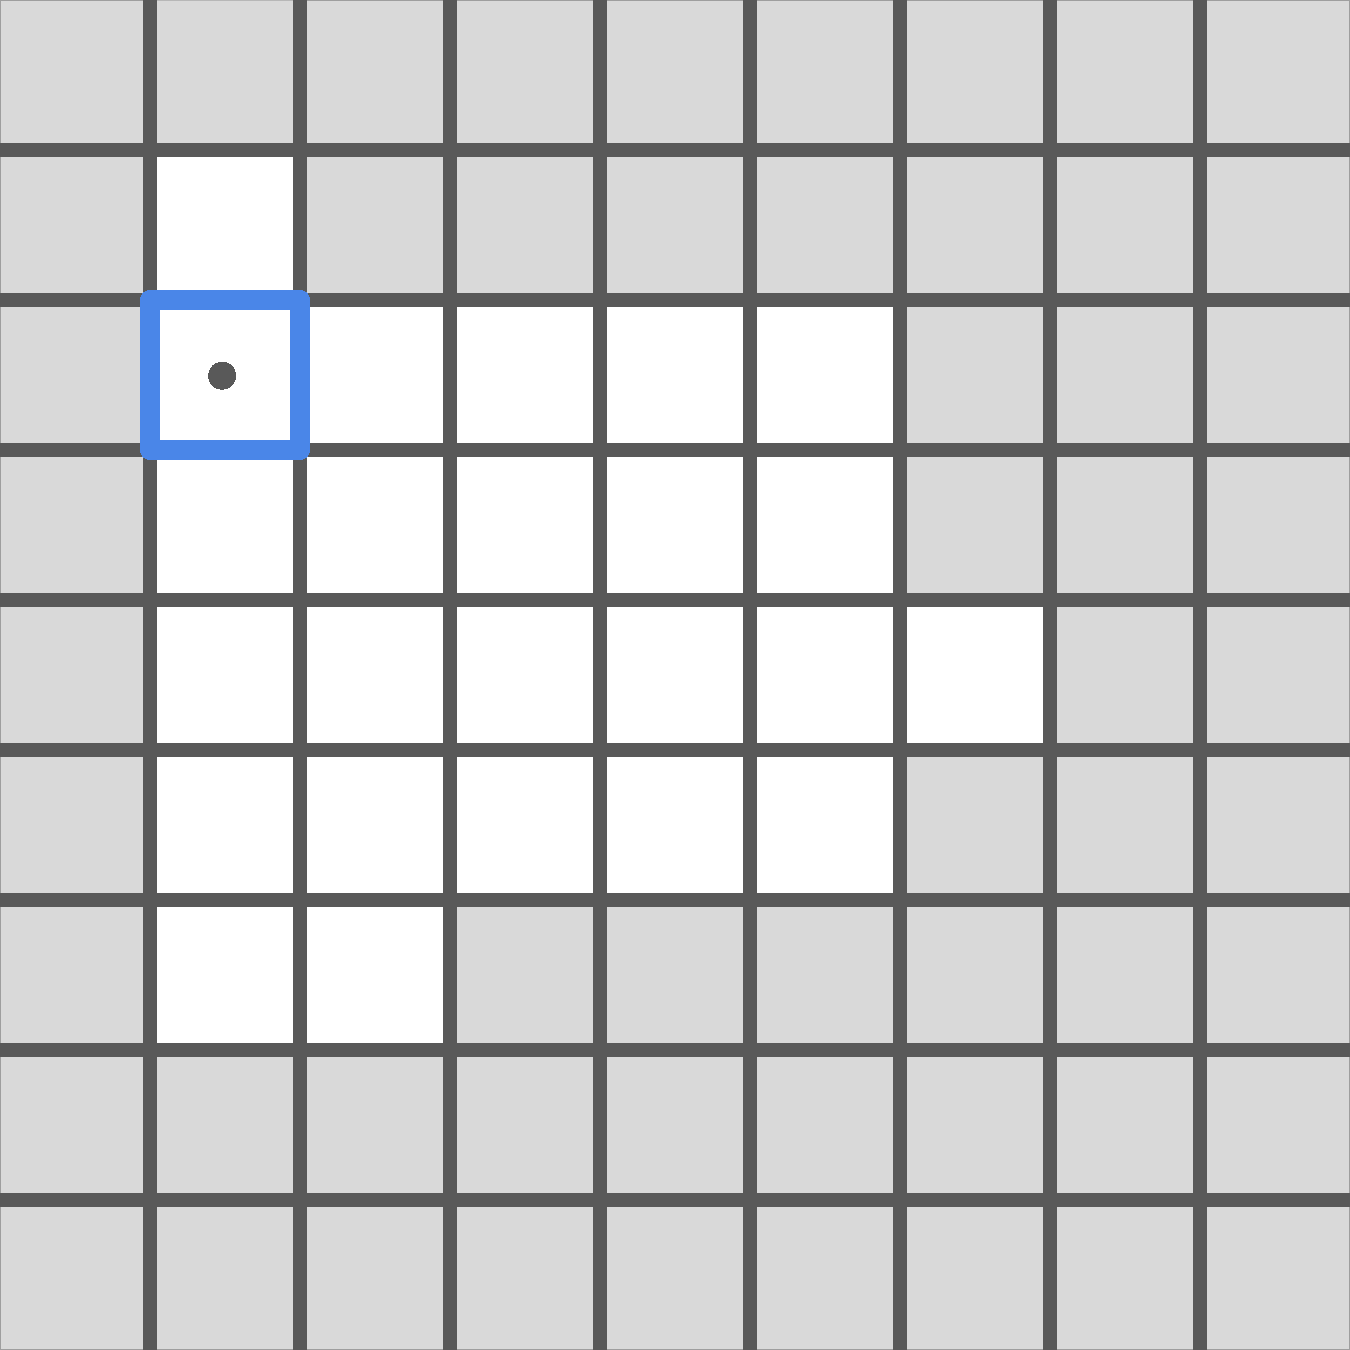
\includegraphics[width=\linewidth,trim={0 100 100 0},clip]{spiker-diagram/spiker-generate}
  \caption{TODO}
  \label{fig:TODO}
\end{subfigure}
\begin{subfigure}[b]{0.33\linewidth}
  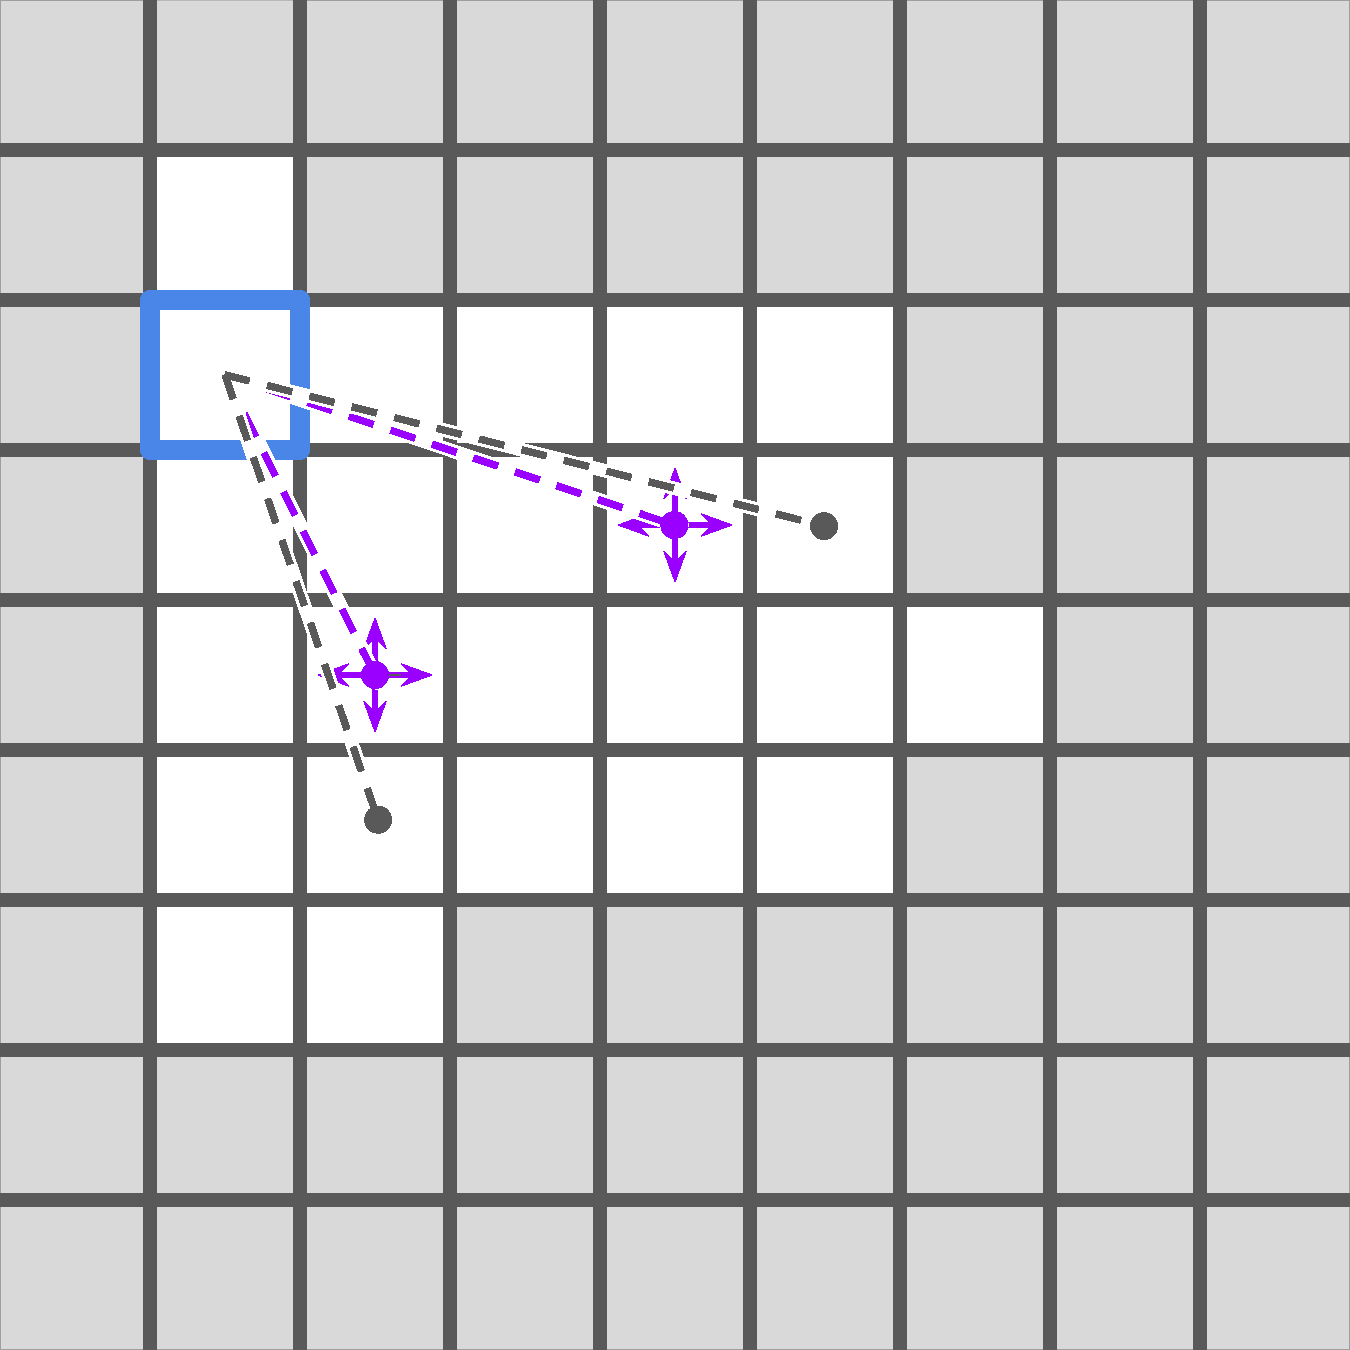
\includegraphics[width=\linewidth,trim={0 100 100 0},clip]{spiker-diagram/spiker-walk}
  \caption{TODO}
  \label{fig:TODO}
\end{subfigure}
\begin{subfigure}[b]{0.33\linewidth}
  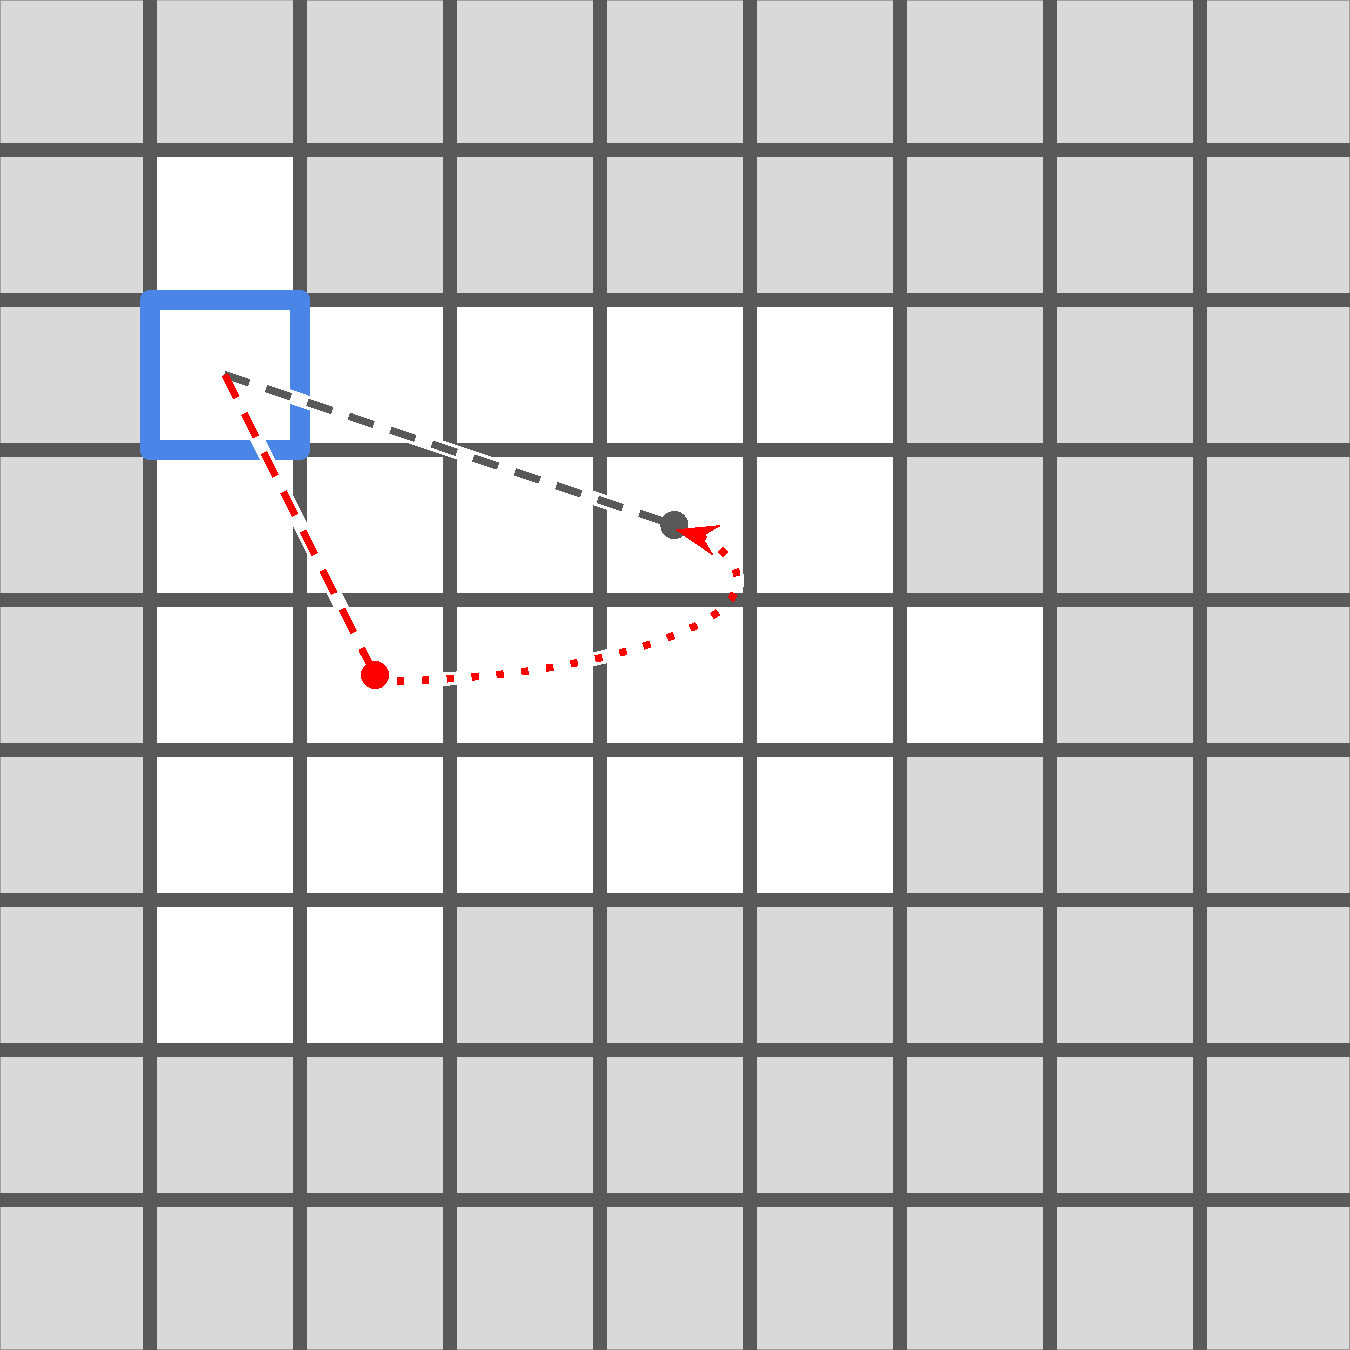
\includegraphics[width=\linewidth,trim={0 100 100 0},clip]{spiker-diagram/spiker-swap}
  \caption{TODO}
  \label{fig:TODO}
\end{subfigure}
\begin{subfigure}[b]{0.33\linewidth}
  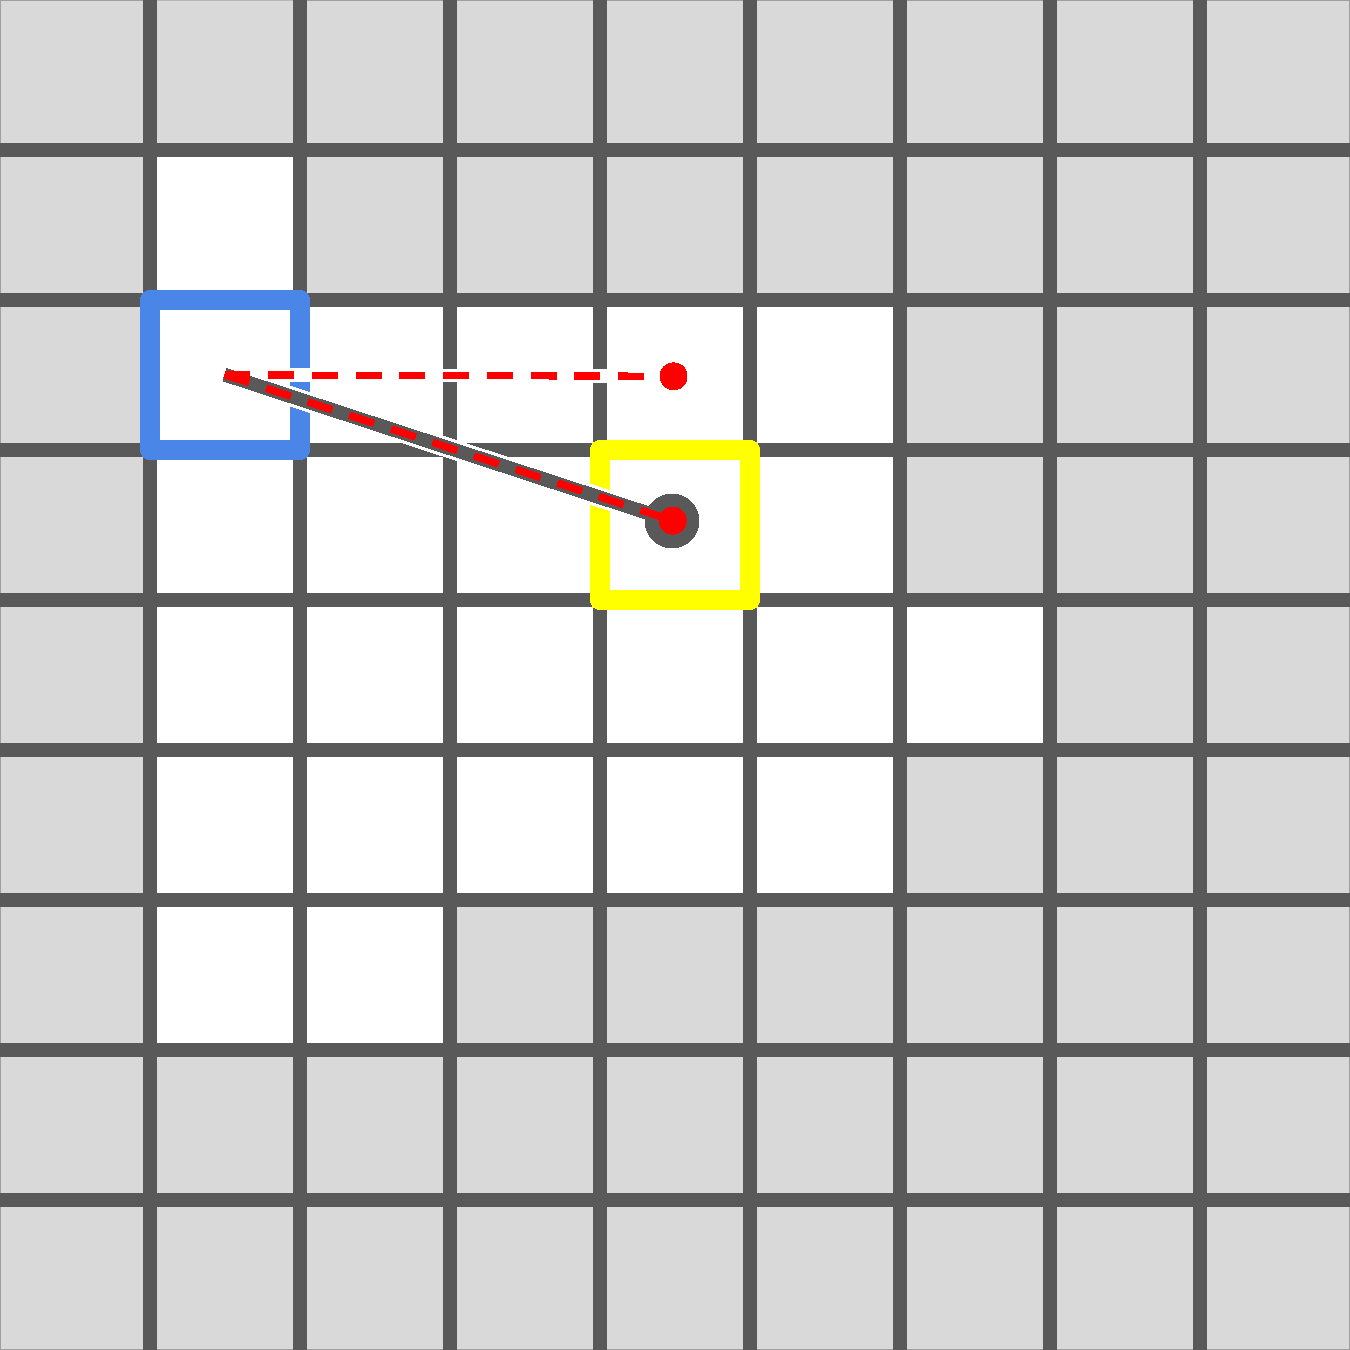
\includegraphics[width=\linewidth,trim={0 100 100 0},clip]{spiker-diagram/spiker-connect}
  \caption{TODO}
  \label{fig:TODO}
\end{subfigure}
\begin{subfigure}[b]{0.33\linewidth}
  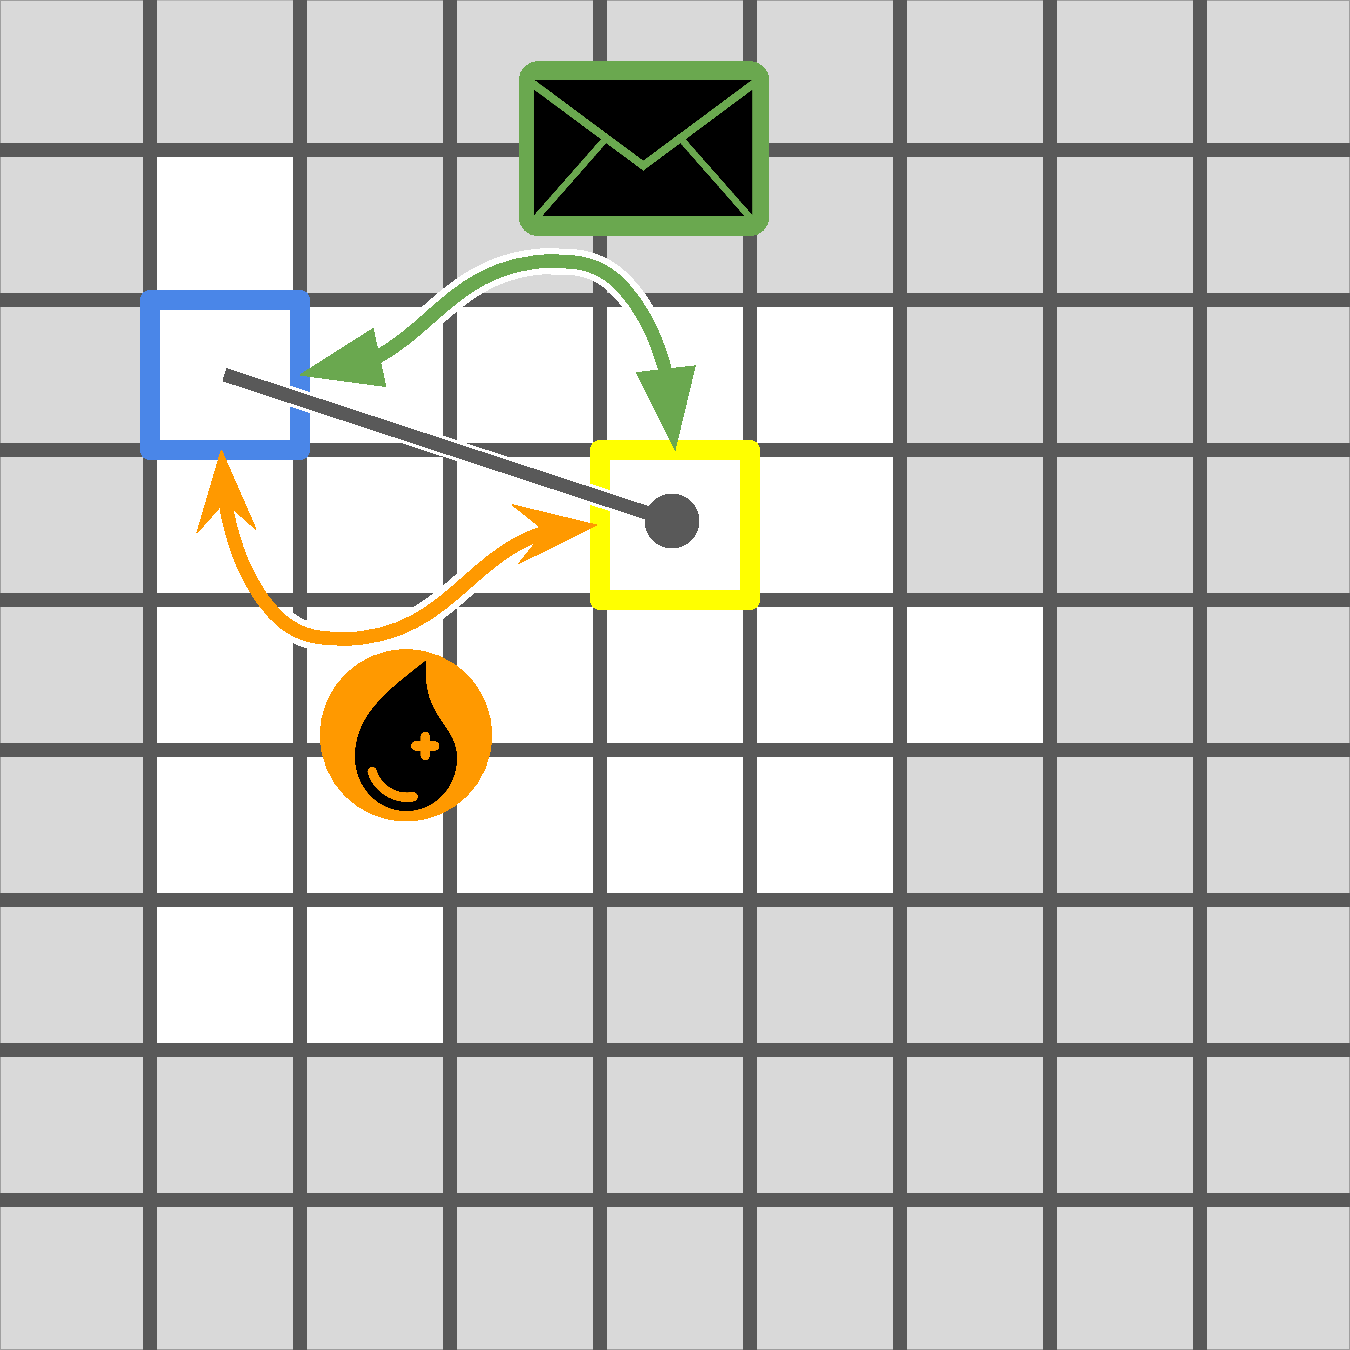
\includegraphics[width=\linewidth,trim={0 100 100 0},clip]{spiker-diagram/spiker-transmit}
  \caption{TODO}
  \label{fig:TODO}
\end{subfigure}
\begin{subfigure}[b]{0.33\linewidth}
  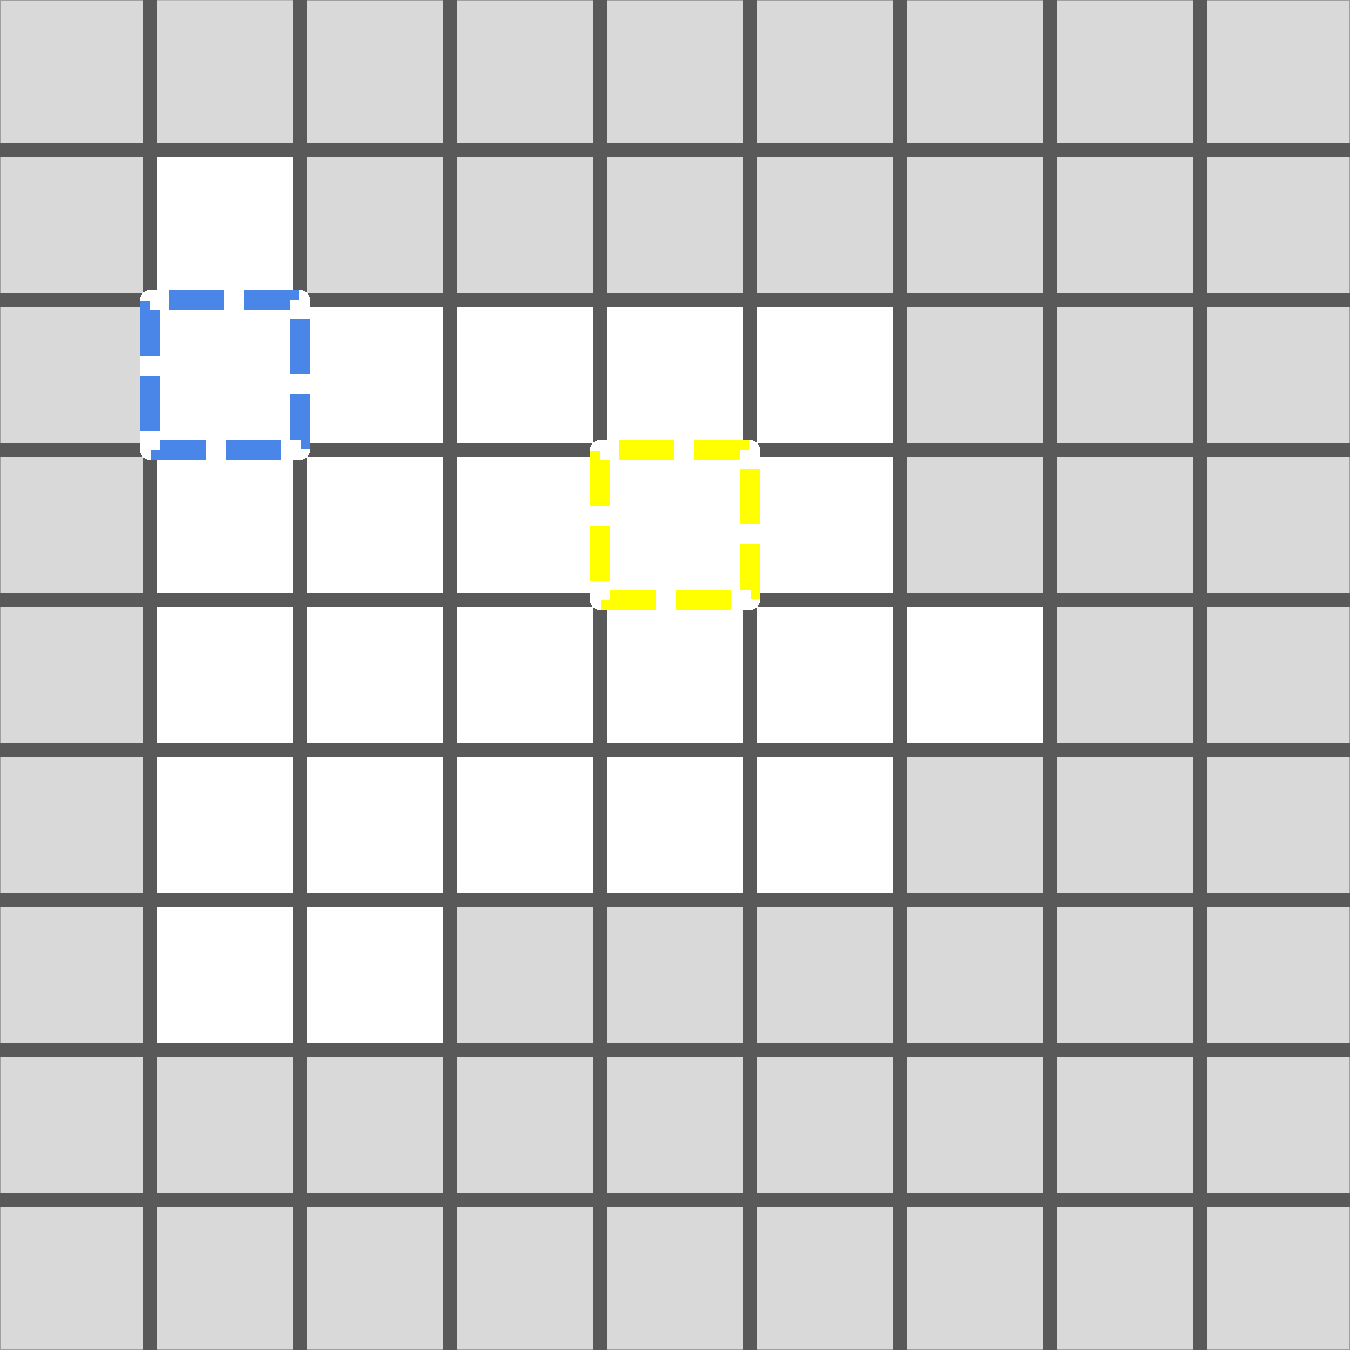
\includegraphics[width=\linewidth,trim={0 100 100 0},clip]{spiker-diagram/spiker-remove}
  \caption{TODO}
  \label{fig:TODO}
\end{subfigure}
\caption{
TODO
}
\label{fig:spiker_diagram}
\end{center}
\end{figure*}


\subsection{Evolutionary Screens}

Our evolutionary screens consisted of 64 independent evolutionary batches.
We processed each batch in four-hour epochs to enable efficient job scheduling.
Each batch consisted of four isolated 45-by-45 toroidal subpopulations.
Subpopulations were completely intermixed in between four-hour steps.
To facilitate evolutionary search, in addition to a base mutation rate applied to cell division, additional mutations were applied to cells seeding a toroidal grid at the outset of an epoch or budding to form new kin groups during an epoch.

We screened across four-hour checkpoints of replicate batches to see if messages or resource were being sent over interconnects.
We sampled from these populations, performing screens for knockouts of over-interconnect messaging or resource sharing.
We then performed a secondary screen on strains with adaptive over-interconnect messaging or resource sharing to determine if re-routing either messages or shared resources decreased fitness.

We measured relative fitness using competition experiments between strains.
For some competition experiments reported in the case studies, we provide hyperlinks to load a in-browser DISHTINY simulation with the actual strains that were used.
In this web viewer, wild-type strains carry phylogentic root ID 1 and knockout strains carry ID 2.

\subsection{Implementation}

We implemented our experimental system using the Empirical library for scientific software development in C++, available at \url{https://github.com/devosoft/Empirical} \citep{charles_ofria_2019_2575607}.
We used OpenMP to parallelize our main evolutionary replicates, distributing work over two threads.
The code used to perform and analyze our experiments, our figures, data from our experiments, and a live in-browser demo of our system is available via the Open Science Framework at \url{https://osf.io/53vgh/} \citep{foster2017open}.
